\documentclass[11pt, oneside]{article}   	% use "amsart" instead of "article" for AMSLaTeX format
\usepackage{geometry}                		% See geometry.pdf to learn the layout options. There are lots.
\geometry{letterpaper}                   		% ... or a4paper or a5paper or ... 
\usepackage{graphicx}				% Use pdf, png, jpg, or eps§ with pdflatex; use eps in DVI mode
								% TeX will automatically convert eps --> pdf in pdflatex		
\usepackage{amssymb}
\usepackage{enumitem}
\usepackage{tikz}

\title{COMP2007 - Assignment 3}
\author{Matthew Watson\\ SID: 440267858}
\date{}							% Activate to display a given date or no date

\begin{document}
\maketitle

\begin{enumerate}
	\item \textbf{Design an algorithm that chooses the subset of houses with maximum combined value, given the constraint that no two chosen houses can be adjacent. That is, you can't choose both a house and its neighbour.}
	\begin{enumerate}
		\item \textbf{Design a dynamic programming algorithm to determine the value of the optimal choice of houses. First derive and justify a recurrence relation and your base cases, then turn it into a bottom-up solution. A more efficient algorithm gives more points.}\\
		To determine the optimal choice of houses, we must first derive a recurrence relation. We can define a function $OPT(i)$ as the maximum house value from the first house in our sequence up to and including that of the $i^{th}$ house, and the value of the $i^{th}$ house being $v_i$. When we reach the $i^{th}$ house, there are two options; to add this house to our subset of houses with maximum combined value, or not. This is best explained by the following equation:
		\[OPT(i) = max(v_i + OPT(i-2) \textrm{ when the}\ i^{th} \textrm{house is added,}\ OPT(i-1) \textrm{ otherwise)} \]
		
		From this we can form a bottom-up algorithm that computes the subset of houses with the maximum combined value. The order of our dynamic program will run as follows:
		\begin{enumerate}
			\item Fill an array from the provided house values called \textit{house\_values} and the number of houses represented by \textit{num\_houses}.
			\item Check if the number of houses is zero, in which case the maximum value will be zero.
			\item Check if the number of houses is one, in which case the maximum value is the value of that one house.
			\item Check if the number of houses is two, in which case we can only pick one of these houses as the other is a neighbour. So we find the max of the two values and return that as our maximum value.
			\newpage
			\item Otherwise, we have a sequence of 3 or more houses, and can prepare our algorithm by computing the maximum value of the first two homes and setting that as our variable to keep track of our current maximum value, called \textit{curr\_max\_value}. Then,
			\item We run a for loop from index 2 ($3^{rd}$ house) until index \textit{num\_houses} (the previously calculated number of houses in our sequence).
			\item At each iteration, we simply call on our function to determine whether we pick the house at our current $i^{th}$ iteration. That is, we determine the greater value of the following two cases:
			\begin{itemize}
				\item We chose this house at \textit{i} to be a part of our subset and so the maximum value of such is the value of this house at \textit{i} plus the maximum value up until the last non-adjacent house to \textit{i}, i.e. up until \textit{i-2}. Or,
				\item We don't chose this house at \textit{i} and so the maximum value will be that up until the last adjacent house, i.e. up until \textit{i-1}
			\end{itemize}
			The greater value is then added to our \textit{curr\_max\_value} variable.
			\item With the maximum obtained at house \textit{i}, we iterate through our for loop repeating our function until we have reached the end of our input sequence of houses and then return the last and final value of \textit{curr\_max\_value} to give the combined value of our subset of non-adjacent houses with maximum combined value.
		\end{enumerate}
		\newpage
		\item \textbf{Argue the correctness of your algorithm.}
		\begin{enumerate}
			\item Case where $n=0$: If there are no houses to visit, then there is 0 value and hence the final value is 0 as there can be no other houses to add value.
			\item Case where $n=1$: If there is only one house, then the optimum value will be the value of this house, $v_i$ as there would be no other houses to add value.
			\item Case where $n=2$: If there are only two houses, then finding the optimum value will simply be the maximum value between these two houses as selecting none would give no value and both can't be selected as they cannot be adjacent. Hence the max value of the two houses where $n=2$ is the optimum value.\\
			\\
			\textbf{Proof for n}
			\item Case where $n=7$:\\
			\\
			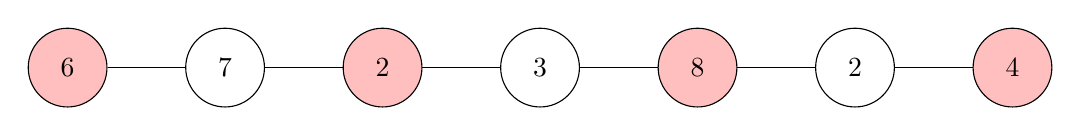
\begin{tikzpicture}
				\node[circle,draw, minimum size=1cm, fill=pink] (A) at  (0,0) {6};
				\node[circle,draw, minimum size=1cm] (B) at  (2,0)  {7};
				\draw (A) -- (B);
				\node[circle,draw, minimum size=1cm, fill=pink] (C) at  (4,0) {2};
				\draw (B) -- (C);
				\node[circle,draw, minimum size=1cm] (D) at  (6,0)  {3};
				\draw (C) -- (D);
				\node[circle,draw, minimum size=1cm, fill=pink] (E) at  (8,0)  {8};
				\draw (D) -- (E);
				\node[circle,draw, minimum size=1cm] (F) at (10,0) {2};
				\draw (E) -- (F);
				\node[circle,draw, minimum size=1cm, fill=pink] (G) at (12,0) {4};
				\draw (F) -- (G);
			\end{tikzpicture}\\
			The algorithm will start at the beginning of the list and compare the optimum values of $v_i + v_{i-2}$ (seen below on the left) and $v_{i-1}$ (seen below on the right) until the list has been iterated through. See the following for an example iteration on the above houses list.
			\begin{itemize}
				\item $h1$ = 6
				\item $h2$ = $6\; |\; \textbf{7}$
				\item $h3$ = $\textbf{2+6}\:|| \:7$
				\item $h4$ = $\textbf{3+7}\:|| \:8$
				\item $h5$ = $\textbf{8+2+6}\:|| \:3+7$
				\item $h6$ = $2+3+7\:|| \:\textbf{8+2+6}$
				\item $h7$ = $\textbf{4+8+2+6}\:|| \:2+3+7$
			\end{itemize}
			Thus the value of our subset of houses of maximum combined value is $4+8+2+6=20$ which is the correct value of the 7 houses. As this continues for all sizes n, we conclude this algorithm is correct.
			
		\newpage	
		\end{enumerate}
		\item \textbf{Prove an upper bound on the time complexity of your algorithm}\\
		We first read in a sequence of house values that are appended to a list. Appending to a list takes $O(1)$ time and is repeated n times. This means $O(N)$ overall time for the data input. We then begin our algorithm. If the number of houses is 0, we return 0 in $O(1)$ time. If the number of houses is 1, we return the value at index 0 from \textit{house\_values} in $O(1)$ time. If the number of houses is 2, we simply return the max of the two houses. Retrieval of two values from a list is $O(1)$ time done twice to be $O(1)$ overall. The max operator on two numbers takes $O(1)$ time and so combined with the list retrieval, this step takes $O(1)$ time. Now that our edge cases are covered, we can initialise our \textit{curr\_max\_value} variable and append the first house as the max value at index 0 and then the max of the first and second houses as the max value at index 1. Appending to a list is $O(1)$ time as well as our max operation making this $O(1)$ time overall. With this done, we enter a for loop from $i=2$ to n. On each iteration we get the current house value and the $i-1$ and $i-2$ value from \textit{curr\_max\_value} each in $O(1)$ time. We call max on the formula of these as outlined above and so is $O(1)$ overall. We can conclude our for loop hence takes $O(N)$ time. Finally we can calculate the overall time complexity:
		\[ O(N) + O(1) + O(1) + O(1) + O(1) + O(1) + O(N)\]
		\[ = O(N) \]
	\end{enumerate}
	\newpage
	\item \textbf{Find the subset S $\subset$ V that maximises the sum of node values, given that no two nodes in S can be connected by an edge}
	
	\begin{enumerate}
		\item \textbf{Design a dynamic programming algorithm to determine the value of the optimal choice of houses. First derive and justify a recurrence relation and your base cases, then turn it into a bottom-up solution. A more efficient algorithm gives more points.}\\
		To determine the optimal choice of houses, we must first derive a recurrence relation. We can define a function $OPT(i)$ as the value of the optimal choice of houses in our sequence up to and including that of the $i^{th}$ house, where the value of the $i^{th}$ house being $v_i$. When we reach the $i^{th}$ house, there are two options, to add this house to our subset of houses with maximum combined value, or not. This is best explained by the following equation:
		\[OPT(i) = max((v_i + OPT[\textrm{left}] + OPT[\textrm{right}]), (OPT[\textrm{left's children}] + OPT[\textrm{right's children}])) \]
		
		This is because no two nodes in S can be connected by an edge; such that we can either pick the optimum of the children, or the optimum of the grand children plus current house $i$.
		
		From this we can now form a bottom-up algorithm that computes the subset of houses with the maximum combined value. The order of our dynamic program will run as follows:
		\begin{enumerate}
			\item Fill a list of nodes from the input to represent our full binary tree of houses
			\item Initialise two arrays to hold our optimal include and exclude values. Include will keep track of the optimum value of the current node $i$ and its grand children. Exclude will keep track of the optimum value of the children.
			\item Iterate through the list of nodes starting at the end going backwards toward the start. In relation to the tree structure, this means starting at the bottom right-most node and ending at the top root node. 
			\item If current node $i$ has not got children or grand children (i.e. if the child node index formula runs out of bounds), then only fill the include max value with the current value $v_i$ (as there are no grand children) and leave the exclude value as 0 as there are no children.
			\item Once the iteration reaches nodes with children and/or grand children, calculate the maximum exclude value by adding the maximum of the left and right children as well as the maximum include value by adding the value of the current node $i$ plus the maximum of the left and right grand children.
			\item Once the iteration has completed to the top of the tree, take the max value from the include and exclude array at index 0 and return that as the result. This will be the value of the optimal choice of houses.
		\end{enumerate}
		
		\item \textbf{Argue the correctness of your algorithm.}\\
		\begin{enumerate}
			\item Case where $n=0$: If there are no houses to visit, then there is 0 value and hence the final value is 0 as there can be no other houses to add value.
			\item Case where $n=1$: With only one node available, the root is the start node, end node and the only element. Becuase of this, the weight of n + grand children is just n as there are no grand children. Our exclude list will be 0 as there are no children to be added to it. Returning the highest sum of this subset will be the highest value.
			\item Case where $n=2$: If there are only two houses, then finding the optimum value will simply be the maximum value between these two houses as selecting none would give no value and both can't be selected as they cannot be adjacent. Hence the max value of the two houses where $n=2$ is the optimum value.\\
			\\
			\textbf{Proof for n}
			\item Case where $n=3$:\\
			\\
			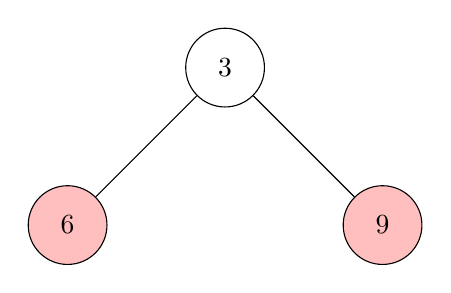
\begin{tikzpicture}
				\node[circle,draw, minimum size=1cm, fill=pink] (A) at  (0,0) {6};
				\node[circle,draw, minimum size=1cm] (B) at  (2,2)  {3};
				\draw (A) -- (B);
				\node[circle,draw, minimum size=1cm, fill=pink] (C) at  (4,0) {9};
				\draw (B) -- (C);
			\end{tikzpicture}\\
			\begin{itemize}
				\item $node2$ = $\textbf{9}\:|| \:0$
				\item $node1$ = $\textbf{6}\; |\; 0$
				\item $node0$ = $3\:|| \:\textbf{6+9}$
			\end{itemize}
			Node 0 is the root and node 1 and 2 are node 0's children. Nodes 1 and 2 will have an include summation of 6 and 9 respectively, with an exclude summation of 0 as neither of them have children. Node 0 will have an include summation of itself and the grand children (of which there are none) hence totalling 3. Node 0 will have an exclude of the optimum of the children which is 15. Hence, the optimum sum of the nodes in this tree will be 15 which is from our final subset of maximum value of houses such that no two nodes can be connected by an edge.
			\newpage
			\item Case where $n=7$:\\
			\\
			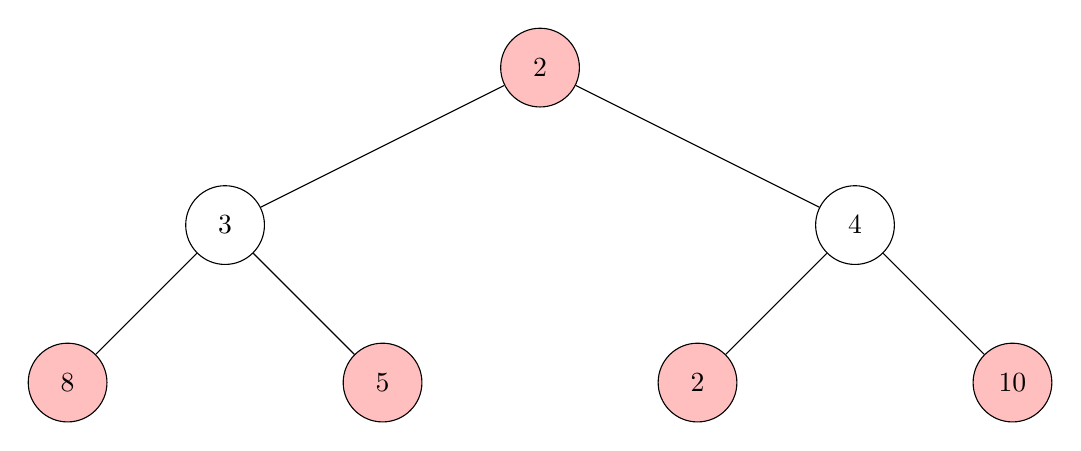
\begin{tikzpicture}
				\node[circle,draw, minimum size=1cm, fill=pink] (A) at  (0,0) {2};
				\node[circle,draw, minimum size=1cm] (B) at  (-4,-2)  {3};
				\draw (A) -- (B);
				\node[circle,draw, minimum size=1cm] (C) at  (4,-2) {4};
				\draw (A) -- (C);
				\node[circle,draw, minimum size=1cm, fill=pink] (D) at  (-6,-4) {8};
				\draw (B) -- (D);
				\node[circle,draw, minimum size=1cm, fill=pink] (E) at  (-2,-4) {5};
				\draw (B) -- (E);
				\node[circle,draw, minimum size=1cm, fill=pink] (F) at  (2,-4) {2};
				\draw (C) -- (F);
				\node[circle,draw, minimum size=1cm, fill=pink] (G) at  (6,-4) {10};
				\draw (C) -- (G);
			\end{tikzpicture}\\
			\begin{itemize}
				\item $node6$ = $\textbf{10}\:|| \:0$
				\item $node5$ = $\textbf{2}\:|| \:0$
				\item $node4$ = $\textbf{5}\:|| \:0$
				\item $node3$ = $\textbf{8}\:|| \:0$
				\item $node2$ = $4\;|| \;\textbf{2+10}$
				\item $node1$ = $3\;|| \;\textbf{8+5}$
				\item $node0$ = $\textbf{2+(10+2+5+8)}\:|| \:3+4$
			\end{itemize}
			Here, we see the last 4 nodes \textit{node6, node5, node4, node3} with values 10, 2, 5 and 8 respectively in the list are leaf nodes (no children). The 2 prior to them, \textit{node2} and \textit{node1} with values 4 and 3 respectively, are the parents of \textit{(node6 \& node5)} and \textit{(node4 \& node3)} respectively. Finally \textit{node0} with value 2 is the root node with children \textit{node1 \& node2}. For nodes 6,5,4 and 3, they will all pick each other as the optimum as they have no children nor grand children to compare to. Stepping into \textit{node2} with value 4, it will compare its include of 4+0 (as it has no grandchildren) and its exclude of \textit{(node6 \& node5)} with values 10 and 2 respectively. As $10+2>4$, the exclude will be chosen as optimal. Same with \textit{node1} where its exclude of values 5 and 8 will sum to be greater than its include value of itself and so the exclude will be chosen. Finally at \textit{node0}, it will compare its include (the value of itself, 2, and the optimum of its grand children, $8+5+2+10=25$) and its exclude, the optimum of its children, $2+4=6$. As $25>5$, the include will be chosen. As this is the root node, the algorithm exits returning what it has proven to be the value of the subset of the optimum choices of houses with maximum value.
			
		\end{enumerate}

		\newpage		
		\item \textbf{Prove an upper bound on the time complexity of your algorithm.}\\
		We first read in a sequence of house values that are appended to a list. Appending to a list takes $O(1)$ time and is repeated n times. This means $O(N)$ overall time for the data input. We then begin our algorithm. The algorithm is contained in a for loop that is iterates N times. Contained in this for loop are several instances of accessing values from a list in $O(1)$ time calling the max function on these also in $O(1)$ time. Thus, the for loop takes $O(N)$ time overall. Finally, to calculate the solution value, we retrieve two values from a list in $O(1)$ time and then call max on these values, also in $O(1)$ time. Finally we can calculate the overall time complexity:
		\[ O(N) + O(N) + O(1)\]
		\[ = O(N) \]

		
		\end{enumerate}

\end{enumerate}
\end{document}  \documentclass[fontsize=12pt, paper=a4]{scrlttr2}

